% Provenance (never printed): see sources/outline_sources.md (Year 1:
% observational astronomy, photometry). Telescopes, angular resolution,
% gratings, the Doppler effect and the black-body laws are owned by the
% physics series and recalled here. Curves computed in
% figdata/bachelor-1/{blackbody_bands, extinction_line}.py; numbers of the
% exercises and problem in the Book 3 scratch calculator ch02.py.
\chapter{Teleskop, detektor dan fotometri}\label{ch:b1:observing-the-sky}

Hampir semua yang diketahui astronomi tentang bintang, selain sejumlah meteorit dan sampel yang dibawa pulang dari Bulan dan asteroid, diperolehnya dari cahaya yang dikirimkan bintang-bintang itu. Cahaya itu melintasi atmosfer Bumi, yang menyerap seluruh rentang panjang gelombang dan mengaburkan sisanya; ia dikumpulkan oleh cermin yang ukurannya membatasi seberapa redup dan seberapa halus rincian yang dapat terlihat; ia dihitung oleh detektor yang mengubah foton menjadi elektron, dan setiap hitungan membawa ketidakpastian statistik. Sebelum kecerahan menjadi \omterm{def:b1:observing-the-sky:flux}{luminositas} atau jarak, setiap langkah ini harus dipahami dan dikoreksi. Bab ini mengikuti cahaya dari bintang sampai menjadi angka: jendela-jendela atmosfer dan hukum ekstingsi, teleskop dan \omterm{def:b1:observing-the-sky:seeing}{kekaburan atmosfer}, detektor dan deraunya, lalu magnitudo, paralaks dan warna yang mengubah \omterm{def:b1:observing-the-sky:flux}{fluks} terukur menjadi sifat-sifat bintang. Atmosfer yang sama, bila dilihat dari bawah, menjadi pokok bab-bab iklim (\cref{ch:b1:radiation-heat-transport}); fotometri yang sama, bila diterapkan pada planet, membuka bab berikutnya (\cref{ch:b1:comparative-planetology}).

\begin{recall}
Objektif teleskop mengumpulkan cahaya di atas aperturnya dan membentuk bayangan di titik fokusnya; difraksi oleh apertur berdiameter $D$ membatasi sudut terkecil yang dapat dipisahkannya menjadi sekitar $1.22\,\lambda/D$, yaitu kriteria Rayleigh (volume Sarjana Tahun ke-1 buku fisika). Kisi menguraikan cahaya menurut panjang gelombang (Sarjana Tahun ke-2), dan sumber yang bergerak sepanjang garis pandang menggeser garis spektrumnya karena efek Doppler (kelas 12). Benda dalam kesetimbangan termal memancarkan spektrum benda hitam, yang puncaknya mengikuti hukum Wien (Sarjana Tahun ke-2). Dalam kimia, absorbansi suatu larutan bertambah sebanding dengan panjang lintasannya.
\end{recall}

\section{Jendela atmosfer}

Atmosfer transparan terhadap sebagian panjang gelombang dan buram terhadap sebagian lainnya. Radiasi terutama diserap oleh uap air, karbon dioksida dan ozon, dan pada panjang gelombang terpendek oleh atom dan molekul di atmosfer atas itu sendiri.
% ledger: nasa:ems-absorbers

\begin{definition}[Jendela atmosfer]\label{def:b1:observing-the-sky:window}
Yang disebut \emph{jendela atmosfer}\index{jendela atmosfer} adalah rentang panjang gelombang tempat atmosfer meneruskan sebagian besar radiasi yang sampai di puncaknya hingga ke permukaan tanah. \emph{Jendela optik} membentang dari ultraviolet dekat sampai inframerah dekat; \emph{jendela radio} dari panjang gelombang sekitar satu sentimeter sampai sekitar sepuluh meter.
\end{definition}

Gambar di bawah ini memperlihatkan opasitas atmosfer dari sinar gamma sampai gelombang radio panjang. Sinar gamma, sinar-X, dan ultraviolet di bawah sekitar \qty{0.3}{\micro\metre} tidak pernah mencapai permukaan tanah: ia diamati dari angkasa. Cahaya tampak melintas, dengan sedikit \omterm{def:b1:observing-the-sky:seeing}{kekaburan}. Sebagian besar inframerah diserap oleh uap air dan karbon dioksida, kecuali pada jendela-jendela sempit yang dimanfaatkan observatorium darat di tempat tinggi dan kering; \omterm{def:b1:observing-the-sky:magnitude}{pita fotometrik} inframerah dekat berada di dalamnya, pada \qty{1.24}{\micro\metre}, \qty{1.65}{\micro\metre} dan \qty{2.16}{\micro\metre}. Panjang gelombang dari sekitar \qty{30}{\micro\metre} sampai satu milimeter terhalang lagi; gelombang radio dari beberapa sentimeter sampai sekitar sepuluh meter melintas, bahkan melalui awan; yang lebih panjang dipantulkan oleh ionosfer.
% ledger: nasa:opacity-windows, baldry:2mass-pivot

\begin{omfigure}
\begin{tikzpicture}[x=1.0cm, y=2.2cm, font=\scriptsize]
% x = log10(lambda / 1 m) + 10 ; opacity 0..1 (schematic, after the NASA figure)
\fill[omSea!20] (0,0) rectangle (13,1.05);
\fill[brown!50] (0,0) -- (0,1) -- (3.45,1) -- (3.52,0.05) -- (4.03,0.05)
  -- (4.06,0.6) -- (4.09,0.15) -- (4.15,0.6) -- (4.22,0.15) -- (4.28,0.6)
  -- (4.34,0.15) -- (4.42,0.7) -- (4.55,0.25) -- (4.65,0.8) -- (4.9,0.2)
  -- (5.12,0.2) -- (5.25,0.7) -- (5.4,1) -- (7.0,1) -- (7.3,0.6) -- (7.6,0.75)
  -- (8.0,0.5) -- (8.5,0.03) -- (11.0,0.03) -- (11.3,1) -- (13,1) -- (13,0)
  -- cycle;
\draw[black!70] (0,0) rectangle (13,1.05);
\foreach \x in {0,...,13} { \draw (\x,0) -- (\x,-0.05); }
\foreach \x/\l in {0/0.1 nm, 2/10 nm, 4/1 \unit{\micro m}, 6/100 \unit{\micro m}, 8/1 cm,
  10/1 m, 12/100 m}
  { \node[below] at (\x,-0.05) {\l}; }
\foreach \y/\l in {0/0, 0.5/50, 1/100}
  { \draw (0,\y) -- (-0.1,\y); \node[left] at (-0.1,\y) {\l}; }
  \node[rotate=90] at (-0.75,0.5) {opasitas (\%)};
  \node at (6.5,-0.42) {\small panjang gelombang (skala logaritmik)};
  \node[align=center] at (1.7,0.75) {sinar gamma, sinar-X,\\ ultraviolet};
  \node[align=center] at (6.2,0.75) {inframerah\\ jauh};
  \node[align=center] at (9.75,0.5) {jendela radio};
\node[omThm] at (4.15,0.86) {J H K};
  \draw[-{Stealth}] (2.6,1.25) node[above] {jendela optik} -- (3.75,1.07);
  \draw[-{Stealth}] (5.9,1.25) node[above] {jendela inframerah} -- (4.6,1.07);
\end{tikzpicture}

{\small Opasitas atmosfer terhadap radiasi yang datang dari angkasa, dari \qty{0.1}{nm} sampai \qty{1}{km} (skala logaritmik). Skematis, mengikuti gambar NASA berdomain publik: di sini hanya jendela-jendelanya yang penting, bukan bentuk tepat setiap pita serapan. J, H dan K menandai \omterm{def:b1:observing-the-sky:magnitude}{pita fotometrik} inframerah dekat.}
% ledger: nasa:opacity-windows, nasa:ems-absorbers, baldry:2mass-pivot
\end{omfigure}

\subsection*{Ekstingsi}

Bahkan di dalam jendela optik atmosfer menghilangkan sebagian cahaya, melalui serapan dan melalui hamburan oleh molekul dan aerosol. Lapisan tipis dengan tebal $\mathrm ds$ sepanjang sinar menghilangkan sebagian intensitas yang sebanding dengan $\mathrm ds$: $\mathrm dI = -\kappa I\,\mathrm ds$, dengan koefisien ekstingsi $\kappa$ (per meter) yang bergantung pada panjang gelombang dan pada komposisi udara di ketinggian itu. Ini adalah hukum absorbansi larutan, yang diterapkan pada sebuah kolom udara.

\begin{proposition}[Hukum Bouguer]\label{prop:b1:observing-the-sky:bouguer}
Sepanjang sinar yang melewati medium penyerap, intensitas berkurang menurut
\[
  I = I_0\,e^{-\tau}, \qquad \tau = \int_0^s \kappa\,\mathrm ds' ,
\]
dengan $I_0$ intensitas yang memasuki medium dan $\tau$, kedalaman optik lintasan, adalah bilangan murni.
Untuk atmosfer sejajar-bidang, bintang pada jarak \omterm{def:b1:spherical-astronomy:celestial-sphere}{zenit} $z$ (sudut antara arahnya dan vertikal) diamati melalui kedalaman optik $\tau(z) = \tau_0\sec z$, dengan $\tau_0$ kedalaman optik di \omterm{def:b1:spherical-astronomy:celestial-sphere}{zenit}.
\end{proposition}

\begin{proof}
Persamaan $\mathrm dI/I = -\kappa\,\mathrm ds$ dapat dipisahkan: mengintegralkan dari puncak atmosfer ($I = I_0$, $s = 0$) sampai pengamat memberikan
$\ln(I/I_0) = -\int_0^s\kappa\,\mathrm ds'$. Dalam atmosfer sejajar-bidang $\kappa$ hanya bergantung pada ketinggian $y$, dan sinar yang miring sebesar $z$ terhadap vertikal menempuh $\mathrm ds = \mathrm dy/\cos z$ untuk naik sejauh $\mathrm dy$. Maka
$\tau(z) = \int \kappa(y)\,\mathrm dy/\cos z = \tau_0\sec z$.
\end{proof}

\begin{definition}[Massa udara, koefisien ekstingsi atmosfer]\label{def:b1:observing-the-sky:extinction}
Yang disebut \emph{massa udara}\index{massa udara} $X$ suatu pengamatan adalah kedalaman optik garis pandang dibagi kedalaman optik di \omterm{def:b1:spherical-astronomy:celestial-sphere}{zenit}: $X = \tau(z)/\tau_0$. Nilainya 1 di \omterm{def:b1:spherical-astronomy:celestial-sphere}{zenit} dan, untuk atmosfer sejajar-bidang, $X = \sec z$. \emph{Koefisien ekstingsi atmosfer}\index{koefisien ekstingsi atmosfer} $k$ pada suatu pita adalah peredupan, dalam magnitudo, yang dihasilkan oleh satu massa udara, sehingga bintang bermagnitudo $m_0$ di atas atmosfer diamati pada
\[
  m = m_0 + kX .
\]
\end{definition}

Magnitudo didefinisikan dalam \cref{sec:b1:observing-the-sky:magnitudes}; yang diperlukan di sini hanyalah bahwa peredupan dengan faktor $e^{-\tau}$ menambah $2.5\log_{10}e\;\tau = 1.086\,\tau$ magnitudo, sehingga $k = 1.086\,\tau_0$. \omterm{def:b1:observing-the-sky:extinction}{Massa udara} atmosfer sejajar-bidang sangat baik sampai ketinggian sekitar \ang{30} ($X = 2$) dan gagal di dekat cakrawala, tempat $\sec z$ tumbuh tanpa batas sementara lintasan sebenarnya melalui atmosfer yang melengkung tetap berhingga; pengamat menghindari ketinggian rendah karena alasan itu dan karena \omterm{def:b1:observing-the-sky:seeing}{kekaburan} yang bertambah seiring panjang lintasan.

\begin{method}[Garis ekstingsi]\label{met:b1:observing-the-sky:extinction-line}
Untuk mencari magnitudo $m_0$ yang akan dimiliki bintang di atas atmosfer:
\begin{enumerate}
  \item ukurlah magnitudo $m$ bintang, atau bintang standar, pada beberapa \omterm{def:b1:observing-the-sky:extinction}{massa udara} sepanjang malam, saat ia terbit atau terbenam;
  \item hitunglah setiap \omterm{def:b1:observing-the-sky:extinction}{massa udara} dari jarak \omterm{def:b1:spherical-astronomy:celestial-sphere}{zenit}, $X = \sec z$;
  \item gambarkan $m$ terhadap $X$ dan cocokkan garis lurus dengan kuadrat terkecil;
  \item kemiringan garis adalah koefisien ekstingsi $k$ malam itu pada pita tersebut; perpotongannya pada $X = 0$ adalah $m_0$.
\end{enumerate}
Koefisien $k$ yang sama kemudian mengoreksi setiap bintang lain yang diamati malam itu pada pita yang sama: $m_0 = m - kX$.
\end{method}

\begin{example}
Pada suatu malam, sebuah bintang diukur enam kali dalam pita V:
\begin{center}
\small
\begin{tabular}{lcccccc}
\hline
$X$ & 1.05 & 1.18 & 1.36 & 1.62 & 1.95 & 2.31 \\
$m$ & 8.024 & 8.031 & 8.072 & 8.104 & 8.171 & 8.216 \\
\hline
\end{tabular}
\end{center}
Garis kuadrat terkecil, yang digambar pada gambar di bawah, memiliki kemiringan $k = \qty{0.160}{\mag}$ per \omterm{def:b1:observing-the-sky:extinction}{massa udara} dan perpotongan $m_0 = 7.851$. Titik-titiknya tersebar di sekitar garis itu sebesar \num{0.006} magnitudo, ketelitian fotometri malam yang baik. Di \omterm{def:b1:spherical-astronomy:celestial-sphere}{zenit} bintang itu meredup sebesar \num{0.16} magnitudo, kehilangan $1 - 10^{-0.4\times0.160} = \qty{14}{\percent}$ dari cahayanya.
\end{example}

\begin{omfigure}
\begin{tikzpicture}
\begin{axis}[omrecord, width=0.62\linewidth, height=5.4cm, xmin=0, xmax=2.5,
  ymin=7.80, ymax=8.28, y dir=reverse, xlabel={massa udara $X$},
  ylabel={magnitudo $m$}, yticklabel style={/pgf/number format/fixed,
  /pgf/number format/precision=2}, tick label style={font=\scriptsize},
  label style={font=\small}]
\addplot[omThm, line width=0.9pt, dashed] table[x=X, y=m] {figdata/out/bachelor-1-extinction_line-fit.dat};
\addplot[only marks, mark=*, mark size=1.6pt, omDef] table[x=X, y=m] {figdata/out/bachelor-1-extinction_line-obs.dat};
\node[font=\scriptsize, right, fill=white, inner sep=1pt] at (axis cs:0.05,7.83) {$m_0 = 7.851$};
\node[font=\scriptsize, fill=white, inner sep=1pt, rotate=-10] at (axis cs:0.95,8.10) {kemiringan $k = 0.160$};
\end{axis}
\end{tikzpicture}

{\small Garis ekstingsi: magnitudo satu bintang pada enam \omterm{def:b1:observing-the-sky:extinction}{massa udara} (titik-titik) dan garis kuadrat terkecil, diekstrapolasi ke $X = 0$, yaitu magnitudo di atas atmosfer. Magnitudo bertambah ke bawah: bintang yang lebih redup berada lebih rendah.}
\end{omfigure}

\subsection*{Kekaburan atmosfer}

Udara di atas teleskop tidak pernah diam. Sel-sel udara dengan suhu yang sedikit berbeda, dan karena itu indeks bias yang sedikit berbeda, bergeser melintasi berkas dan membelokkannya dengan sudut acak kecil, berubah berkali-kali setiap detik. Mata melihat bintang berkelap-kelip; pemaparan panjang merekam bintik kabur yang jauh lebih besar daripada pola difraksi teleskop.

\begin{definition}[Kekaburan atmosfer]\label{def:b1:observing-the-sky:seeing}
Yang disebut \emph{kekaburan atmosfer}\index{kekaburan atmosfer} di suatu tempat adalah diameter sudut citra sumber titik yang dikaburkan oleh turbulensi atmosfer dalam pemaparan panjang, diukur sebagai lebar penuh citra pada setengah maksimumnya, dalam detik busur.
\end{definition}

\omterm{def:b1:observing-the-sky:seeing}{Kekaburan atmosfer} berubah dari malam ke malam dan dari jam ke jam. Tempat-tempat observasi dipilih berdasarkan hal ini: di puncak Maunakea, pada \qty{4204}{m}, median \omterm{def:b1:observing-the-sky:seeing}{kekaburan atmosfer} bebas kira-kira \ang{;;0.40}, dari sekitar \ang{;;0.45} pada musim dingin sampai \ang{;;0.35} pada musim panas, dengan sepersepuluh malam terbaik di bawah sekitar \ang{;;0.25}; tempat yang sama hanya memiliki median \qty{0.9}{mm} uap air yang dapat mengendap di atasnya, yang membuka jendela inframerahnya.
% ledger: cfht:site, cfht:seeing

\section{Teleskop dan resolusi}

Teleskop melakukan dua hal: ia mengumpulkan cahaya di atas luas objektifnya, dan ia membentuk citra yang rinciannya terpisah. Luas pengumpulan tumbuh sebagai $D^2$: cermin dua kali lebih lebar mengumpulkan empat kali lebih banyak foton dalam waktu yang sama dan menjangkau bintang empat kali lebih redup. Resolusinya dibatasi oleh difraksi sampai sekitar $1.22\,\lambda/D$, dan oleh \omterm{def:b1:observing-the-sky:seeing}{kekaburan atmosfer}.

\begin{example}
Teleskop Canada--France--Hawaii di Maunakea memiliki apertur \qty{3.58}{m}. Pada \qty{550}{nm} batas difraksinya adalah
\[
  1.22\times\frac{\qty{550e-9}{m}}{\qty{3.58}{m}} = \qty{1.87e-7}{rad}
  = \ang{;;0.039},
\]
sepuluh kali lebih halus daripada median \omterm{def:b1:observing-the-sky:seeing}{kekaburan} sebesar \ang{;;0.40} di tempat yang sama. Kedua batas ini sama untuk cermin berdiameter $D = 1.22\lambda/\theta =
1.22\times\qty{550e-9}{m}/(\num{0.40}/\num{206265}) = \qty{0.35}{m}$: setiap teleskop darat yang lebih lebar dari sekitar \qty{35}{cm} dibatasi oleh \omterm{def:b1:observing-the-sky:seeing}{kekaburan atmosfer}, bukan oleh optiknya sendiri, pada panjang gelombang tampak.
% ledger: cfht:aperture, cfht:seeing
\end{example}

Teleskop darat yang besar karena itu memperoleh luas pengumpulan, bukan ketajaman, kecuali ia mengoreksi turbulensi. \emph{Optik adaptif} melakukan hal itu: sebuah sensor mengukur, berkali-kali setiap detik, bagaimana muka gelombang dari bintang terang (atau dari bintang buatan yang dibentuk dengan laser di atmosfer atas) terdistorsi, dan cermin tipis yang dilengkungkan oleh banyak aktuator kecil membatalkan distorsi itu. Koreksi bekerja paling baik di inframerah, tempat turbulensinya lebih lambat dan lebih lemah, dan pada medan kecil di sekitar bintang pemandu. Di angkasa tidak ada \omterm{def:b1:observing-the-sky:seeing}{kekaburan} sama sekali.

\section{Detektor}

Mata mengintegrasikan cahaya selama sebagian kecil detik dan hanya merespons sebagian kecil foton yang masuk ke dalamnya. Pelat fotografi mengintegrasikan cahaya selama berjam-jam tetapi hanya merekam sebagian kecil cahaya. Astronomi modern menggunakan detektor foton yang terbuat dari semikonduktor, tempat setiap foton yang diserap dengan energi yang cukup membebaskan sebuah elektron.

\begin{definition}[Efisiensi kuantum, rasio sinyal terhadap derau]\label{def:b1:observing-the-sky:detector}
Yang disebut \emph{efisiensi kuantum}\index{efisiensi kuantum} $\eta$ suatu detektor pada panjang gelombang tertentu adalah pecahan foton datang yang dicatatnya sebagai fotoelektron: $\eta = N_\mathrm{e}/N_\gamma$. \emph{Rasio sinyal terhadap derau}\index{rasio sinyal terhadap derau} suatu pengukuran adalah sinyal terukur dibagi simpangan bakunya, yaitu ukuran khas kesalahan acaknya.
\end{definition}

\emph{Perangkat terkopel muatan} (CCD) adalah detektor standar jendela optik. Ia berupa lempeng silikon tipis yang dibagi menjadi kisi piksel, masing-masing sebuah sumur potensial yang menyimpan elektron yang dibebaskan oleh foton yang diserap di dalamnya selama pemaparan. Pada akhir pemaparan, tegangan yang diberikan berurutan pada elektroda menggeser muatan dari piksel ke piksel, baris demi baris, ke satu penguat yang mengukurnya satu per satu; citra adalah tabel hitungan. CCD merekam sebagian besar foton yang datang di hampir seluruh cahaya tampak, responsnya sebanding dengan cahaya yang diterima sampai muatan maksimum per piksel (\emph{kapasitas penuh} piksel), dan ia dapat mengintegrasikan selama berjam-jam. Larik inframerah bekerja dengan prinsip yang sama pada semikonduktor lain, dibaca piksel demi piksel.

Foton datang secara acak. Jika suatu sumber rata-rata mengirimkan $N$ fotoelektron selama satu pemaparan, hitungan yang benar-benar tercatat berfluktuasi dari satu pemaparan ke pemaparan berikutnya dengan simpangan baku $\sqrt N$ (statistik Poisson, diterima dari teori peluang: hitungan kejadian langka yang saling bebas).

\begin{proposition}[Derau foton]\label{prop:b1:observing-the-sky:snr}
Ketika derau foton dari sumber itu sendiri mendominasi, sebuah sumber yang memberikan $R$ fotoelektron per detik diukur dalam waktu $t$ dengan \omterm{def:b1:observing-the-sky:detector}{rasio sinyal terhadap derau}
\[
  \mathrm{SNR} = \frac{Rt}{\sqrt{Rt}} = \sqrt{Rt} ;
\]
ia tumbuh sebagai akar kuadrat waktu pemaparan, dan sebanding dengan diameter teleskop (karena $R \propto D^2$). Galat pada magnitudo kemudian adalah
$\sigma_m \approx 1.086/\mathrm{SNR}$.
\end{proposition}

\begin{proof}
Sinyalnya adalah $N = Rt$ dengan simpangan baku $\sqrt N$. Untuk magnitudo, $m = -2.5\log_{10}N + \text{konstanta}$, sehingga galat kecil $\sigma_N$ memberikan $\sigma_m = 2.5\log_{10}e\;\sigma_N/N = 1.086/\mathrm{SNR}$.
\end{proof}

Untuk mengukur magnitudo dengan galat \num{0.01} diperlukan SNR sekitar 109, yaitu sekitar \num{12000} fotoelektron. Untuk sumber yang redup, dua suku lain ikut berperan.
Langit sendiri berpendar, dan setiap piksel citra bintang juga mengumpulkan foton langit, dengan laju $B$; penguat juga menambahkan derau baca $\sigma_r$ pada setiap piksel yang dibaca. Ungkapan lengkapnya,
\[
  \mathrm{SNR} = \frac{Rt}{\sqrt{Rt + Bt + n\sigma_r^2}}
\]
pada $n$ piksel citra, tereduksi menjadi $\sqrt{Rt}$ untuk bintang terang dan menjadi $R\sqrt t/\sqrt B$ untuk sumber yang lebih redup daripada langit. Karena $B$ tumbuh dengan luas cakram \omterm{def:b1:observing-the-sky:seeing}{kekaburan}, \omterm{def:b1:observing-the-sky:seeing}{kekaburan} yang baik menguntungkan dua kali: citra yang lebih tajam memisahkan lebih banyak dan mengumpulkan lebih sedikit langit (\cref{exo:b1:observing-the-sky:11}).

\begin{inthefield}[Semalam di teleskop]
Fotometri dilakukan dengan kalibrasi sama banyaknya dengan bintang-bintang. Sebelum malam tiba, pengamat di observatorium profesional mengambil \emph{bingkai bias} (pemaparan dengan panjang nol, yang merekam offset elektronik setiap piksel) dan \emph{bidang rata} (citra bagian dalam kubah yang diterangi merata, atau langit senja, yang memetakan bagaimana sensitivitas berubah dari piksel ke piksel dan di seluruh medan); citra ilmiah dikoreksi dengan mengurangi bias dan membagi dengan bidang rata. Sepanjang malam, bintang standar dengan magnitudo yang diketahui diamati pada beberapa \omterm{def:b1:observing-the-sky:extinction}{massa udara} untuk menetapkan garis ekstingsi dan titik nol yang mengubah hitungan menjadi magnitudo. Malam disebut \emph{fotometrik} bila ekstingsinya cukup stabil agar koreksi ini berlaku; di puncak Maunakea, \qty{55}{\percent} malam bersifat fotometrik.
% ledger: cfht:nights
\begin{center}
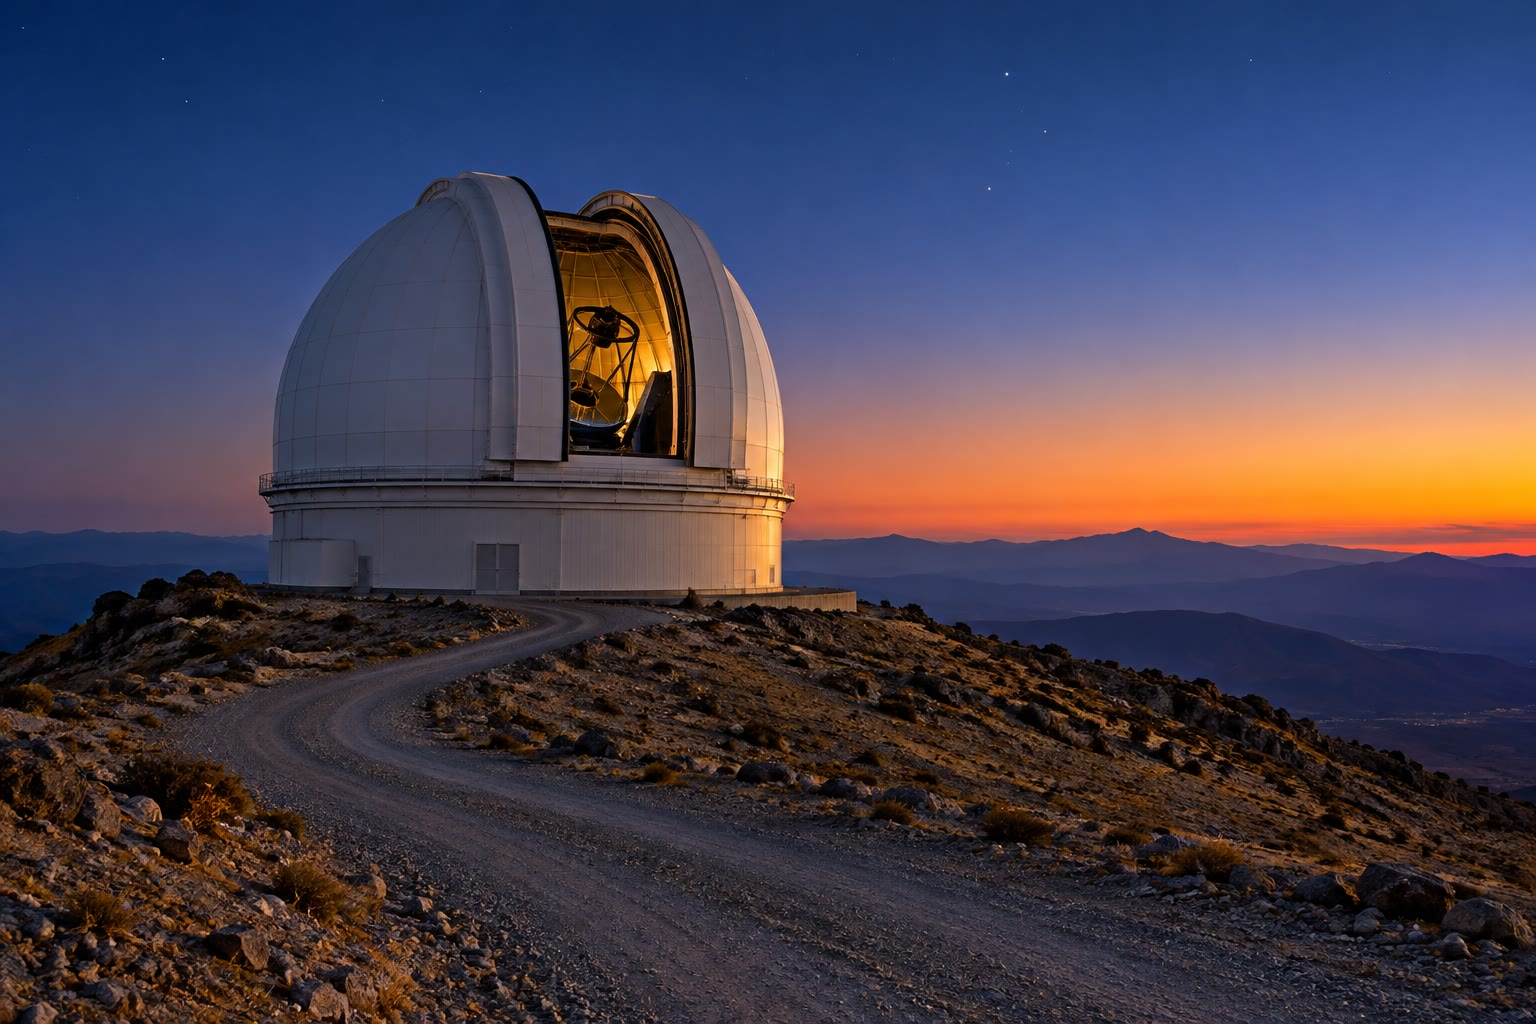
\includegraphics[width=0.55\linewidth]{images/book3/ai/b1-observatory-dusk.jpg}
\end{center}
\end{inthefield}

\section{Fluks dan magnitudo}\label{sec:b1:observing-the-sky:magnitudes}

\begin{definition}[Fluks, luminositas]\label{def:b1:observing-the-sky:flux}
Yang disebut \emph{fluks}\index{fluks (sumber)} $F$ yang diterima dari suatu sumber adalah daya radiasinya yang melintasi satu satuan luas yang dipegang tegak lurus terhadap arahnya, dalam watt per meter persegi; jika dibatasi pada suatu rentang panjang gelombang, ia adalah fluks pada pita itu. \emph{Luminositas}\index{luminositas} $L$ sumber adalah daya total yang dipancarkannya, dalam watt.
\end{definition}

\begin{proposition}[Hukum kuadrat terbalik]\label{prop:b1:observing-the-sky:inverse-square}
Sumber dengan \omterm{def:b1:observing-the-sky:flux}{luminositas} $L$ yang memancar sama ke segala arah, yang diamati pada jarak $d$ melalui ruang hampa, memberikan \omterm{def:b1:observing-the-sky:flux}{fluks}
\[
  F = \frac{L}{4\pi d^2} .
\]
\end{proposition}

\begin{proof}
Dalam keadaan tunak tanpa serapan, daya yang melintasi bola mana pun yang berpusat pada sumber adalah sama, yaitu $L$, menurut kekekalan energi. Karena simetri, daya itu tersebar merata pada luas bola $4\pi d^2$.
\end{proof}

\begin{example}
\omterm{def:b1:observing-the-sky:flux}{Luminositas} Matahari adalah \qty{3.828e26}{W}. Pada satu satuan astronomi, \qty{1.496e11}{m}, \omterm{def:b1:observing-the-sky:flux}{fluksnya} adalah $\num{3.828e26}/(4\pi\times
(\num{1.496e11})^2) = \qty{1361}{W.m^{-2}}$: iradiansi Matahari yang diterima Bumi di puncak atmosfernya.
% ledger: sun:L, const:au, earth:TSI
\end{example}

\omterm{def:b1:observing-the-sky:flux}{Fluks} mencakup rentang yang sangat besar, dan astronom membandingkannya pada skala logaritmik yang diwarisi dari kelas-kelas tempat bintang-bintang yang tampak dengan mata dahulu dikelompokkan: yang paling terang di magnitudo pertama, yang paling redup di magnitudo keenam.

\begin{definition}[Magnitudo tampak, pita fotometrik]\label{def:b1:observing-the-sky:magnitude}
Yang disebut \emph{pita fotometrik}\index{pita fotometrik} adalah rentang panjang gelombang yang dipilih oleh filter standar dan diberi nama dengan huruf: U (ultraviolet), B (biru), V (visual), R (merah), I (inframerah dekat), dan J, H, K pada jendela inframerah. Sebuah \emph{magnitudo tampak}\index{magnitudo tampak} $m$ suatu sumber pada suatu pita didefinisikan dari \omterm{def:b1:observing-the-sky:flux}{fluksnya} $F$ pada pita itu oleh
\[
  m_1 - m_2 = -2.5\log_{10}\frac{F_1}{F_2} ,
\]
dengan titik nol ditentukan oleh bintang standar, mendekati magnitudo bintang Vega pada tiap pita. Selisih 5 magnitudo sama dengan faktor tepat 100 dalam \omterm{def:b1:observing-the-sky:flux}{fluks}; satu magnitudo adalah faktor $100^{1/5} = 2.512$. Sumber yang lebih terang memiliki magnitudo yang lebih kecil, dan dapat bernilai negatif.
\end{definition}

Panjang gelombang pivot filter standar U, B, V, R dan I adalah \qty{358.5}{nm}, \qty{437.1}{nm}, \qty{547.8}{nm}, \qty{650.4}{nm} dan
\qty{802.0}{nm}.
% ledger: baldry:bessell-pivot
Pada pita V, Matahari memiliki \omterm{def:b1:observing-the-sky:magnitude}{magnitudo tampak} $-26.74$, Sirius, bintang paling terang di langit malam, $-1.46$, dan Vega $0.03$. Matahari karena itu $10^{0.4\times(26.74 - 1.46)} = \num{1.29e10}$ kali lebih terang daripada Sirius di langit kita; itu belum mengatakan apa pun tentang mana di antara keduanya yang lebih benderang, yang memerlukan jaraknya.
% ledger: nasa:sun-V, simbad:sirius, simbad:vega

\subsection*{Paralaks dan parsek}

Ketika Bumi mengelilingi Matahari, sebuah bintang dekat tampak bergerak terhadap bintang-bintang latar yang jauh lebih jauh, dengan menelusuri dalam setahun sebuah elips kecil. Gerak semu itu adalah pengukuran jarak bintang yang paling langsung: ia memakai orbit Bumi sebagai garis dasar pengukuran, seperti juru ukur.

\begin{definition}[Paralaks tahunan, parsek]\label{def:b1:observing-the-sky:parallax}
Yang disebut \emph{paralaks tahunan}\index{paralaks tahunan} $p$ suatu bintang adalah sudut yang dibentuk di bintang oleh jari-jari orbit Bumi, satu satuan astronomi, yang dilihat tegak lurus terhadap garis pandang; ia adalah setengah sumbu panjang elips tahunan yang tampak ditelusuri bintang itu. \emph{Parsek}\index{parsek} (\unit{\parsec}) adalah jarak tempat satu satuan astronomi membentuk sudut sebesar satu detik busur:
\[
  \qty{1}{\parsec} = \frac{\qty{1}{\au}}{\tan\ang{;;1}} = \qty{206265}{\au}
  = \qty{3.0857e16}{m} = \qty{3.2616}{\lightyear} .
\]
\end{definition}

Karena $p$ sangat kecil, $\tan p \approx p$ dalam radian, dan jarak langsung mengikuti:
\[
  d = \frac{\qty{1}{\au}}{\tan p} \quad\Longrightarrow\quad
  \frac{d}{\unit{\parsec}} = \frac{1}{p/\text{detik busur}} .
\]
Sirius memiliki paralaks sebesar \ang{;;0.37921}, sehingga ia berada pada $1/0.37921 =
\qty{2.637}{\parsec}$, yaitu \qty{8.60}{\lightyear}. Bahkan bintang-bintang terdekat memiliki paralaks di bawah satu detik busur, lebih kecil daripada \omterm{def:b1:observing-the-sky:seeing}{kekaburan atmosfer}: paralaks ditemukan dari pergeseran pusat citra bintang, yang banyak fotonnya dapat ditentukan jauh lebih teliti daripada lebar citra. Sebuah misi antariksa yang diuraikan di akhir bab ini telah mengukur posisi hampir dua miliar objek dengan cara ini.
% ledger: simbad:sirius, const:au, esa:gaia

\begin{omfigure}
\begin{tikzpicture}[font=\small]
\draw[black!50] (0,0) ellipse (2.0cm and 0.55cm);
\fill[orange!80!black] (0,0) circle (3pt) node[below=3pt] {Matahari};
\fill[blue!70!black] (-2.0,0) circle (2pt) node[left, align=right] {Bumi, enam\\ bulan kemudian};
\fill[blue!70!black] (2.0,0) circle (2pt) node[right] {Bumi};
\fill (0,4.4) circle (1.6pt) node[above] {bintang};
\draw[omDef, thick] (0,0) -- node[right, pos=0.55] {$d$} (0,4.4);
\draw[omThm] (2.0,0) -- (0,4.4);
\draw[omThm, dashed] (-2.0,0) -- (0,4.4);
\draw[thick] (0,0) -- node[above] {\qty{1}{\au}} (2.0,0);
\draw[omThm] (0,3.75) arc[start angle=-90, end angle=-65.6, radius=0.65cm];
\node[omThm] at (0.17,3.38) {$p$};
\end{tikzpicture}

{\small \omterm{def:b1:observing-the-sky:parallax}{Paralaks tahunan} (tidak sesuai skala): dilihat dari bintang, jari-jari orbit Bumi membentuk sudut $p$. Terpisah enam bulan, arah bintang berbeda sebesar $2p$. Sudut sebenarnya untuk bintang terdekat berada di bawah satu detik busur.}
\end{omfigure}

\begin{definition}[Magnitudo mutlak, modulus jarak]\label{def:b1:observing-the-sky:absolute}
Yang disebut \emph{magnitudo mutlak}\index{magnitudo mutlak} $M$ suatu bintang pada suatu pita adalah \omterm{def:b1:observing-the-sky:magnitude}{magnitudo tampak} yang akan dimilikinya pada jarak
\qty{10}{\parsec}, dilihat melalui ruang hampa. Selisih $m - M$ disebut \emph{modulus jarak}\index{modulus jarak}.
\end{definition}

\begin{proposition}[Modulus jarak]\label{prop:b1:observing-the-sky:modulus}
Untuk bintang pada jarak $d$ yang dilihat melalui ruang hampa,
\[
  m - M = 5\log_{10}\frac{d}{\qty{10}{\parsec}} .
\]
Jika cahaya diredupkan dalam perjalanannya sebesar $A$ magnitudo ekstingsi, $m - M = 5\log_{10}(d/\qty{10}{\parsec}) + A$. Pada suatu pita, perbandingan \omterm{def:b1:observing-the-sky:flux}{luminositas} dua bintang adalah $L_1/L_2 = 10^{0.4(M_2 - M_1)}$.
\end{proposition}

\begin{proof}
Menurut hukum kuadrat terbalik, \omterm{def:b1:observing-the-sky:flux}{fluks} pada $d$ dan \omterm{def:b1:observing-the-sky:flux}{fluks} pada \qty{10}{\parsec} berbanding sebagai $F(d)/F(\qty{10}{\parsec}) = (\qty{10}{\parsec}/d)^2$. Definisi magnitudo memberikan $m - M = -2.5\log_{10}(\qty{10}{\parsec}/d)^2
= 5\log_{10}(d/\qty{10}{\parsec})$. Ekstingsi mengalikan \omterm{def:b1:observing-the-sky:flux}{fluks} dengan
$10^{-0.4A}$, yang menambahkan $A$ pada $m$. Pada jarak bersama \qty{10}{\parsec}, \omterm{def:b1:observing-the-sky:flux}{fluks} berbanding sebagai \omterm{def:b1:observing-the-sky:flux}{luminositas}, dan
$M_1 - M_2 = -2.5\log_{10}(L_1/L_2)$.
\end{proof}

Matahari memiliki \omterm{def:b1:observing-the-sky:absolute}{magnitudo mutlak} $M_\odot = 4.83$ dan \omterm{def:b1:observing-the-sky:flux}{luminositas} \qty{3.828e26}{W}. Dengan membandingkan \omterm{def:b1:observing-the-sky:absolute}{magnitudo mutlak} sebuah bintang dalam V dengan milik Matahari, diperoleh \omterm{def:b1:observing-the-sky:flux}{luminositasnya} dalam V dalam satuan Matahari, $L/L_\odot = 10^{0.4(4.83 - M)}$ --- sebuah \omterm{def:b1:observing-the-sky:flux}{luminositas} \emph{pita-V}, karena bintang yang jauh lebih panas atau lebih dingin daripada Matahari memancarkan bagian daya yang berbeda di luar pita V.
% ledger: sun:Mabs, sun:L

\subsection*{Warna}

\begin{definition}[Indeks warna]\label{def:b1:observing-the-sky:colour-index}
Yang disebut \emph{indeks warna}\index{indeks warna} suatu bintang adalah selisih magnitudonya pada dua pita, pita yang lebih biru didahulukan; yang paling banyak dipakai adalah $B - V$. $B - V$ yang kecil atau negatif menandai bintang biru, yang besar menandai bintang merah.
\end{definition}

\omterm{def:b1:observing-the-sky:colour-index}{Indeks warna} tidak bergantung pada jarak, karena hukum kuadrat terbalik meredupkan kedua pita sama; ia mengukur bentuk spektrum, dan karenanya suhu permukaan bintang. Sebuah bintang memancarkan kira-kira seperti benda hitam yang spektrumnya memuncak pada $\lambda_\mathrm{max} = b/T$ (hukum Wien, dengan
$b = \qty{2.898e-3}{m.K}$, diterima dari volume Sarjana Tahun ke-2 buku fisika).
Gambar di bawah ini melukiskan tiga spektrum benda hitam: benda dingin pada \qty{3500}{K} memuncak di inframerah dekat dan memberi lebih banyak \omterm{def:b1:observing-the-sky:flux}{fluks} di V daripada di B; suhu efektif Matahari, \qty{5772}{K}, membuat puncaknya pada \qty{502}{nm}, di antara B dan V; benda pada \qty{10000}{K} memuncak di ultraviolet dan lebih terang di B daripada di V. Rasio radiansi B dan V naik secara mantap dengan suhu, dari \num{0.46} menjadi \num{0.97} dan \num{1.53} untuk ketiga kurva, itulah sebabnya $B - V$ turun ketika $T$ naik.
% ledger: const:b, nasa:sun-Teff, baldry:bessell-pivot

\begin{omfigure}
\begin{tikzpicture}
\begin{axis}[omrecord, width=0.9\linewidth, height=5.8cm, xmin=200, xmax=1500,
  ymin=0, ymax=1.17, xtick={200,400,...,1400}, ytick={0,0.5,1},
  xlabel={panjang gelombang (nm)},
  ylabel={$B_\lambda$ / maksimum}, tick label style={font=\scriptsize},
  label style={font=\small}, legend style={font=\scriptsize, at={(0.5,1.03)},
  anchor=south, draw=none, fill=none}, legend columns=3]
\addplot[red!75!black, line width=1.1pt] table[x=lam_nm, y=t3500] {figdata/out/bachelor-1-blackbody_bands-curves.dat};
\addplot[orange!90!black, line width=1.1pt] table[x=lam_nm, y=t5772] {figdata/out/bachelor-1-blackbody_bands-curves.dat};
\addplot[omDef, line width=1.1pt] table[x=lam_nm, y=t10000] {figdata/out/bachelor-1-blackbody_bands-curves.dat};
\legend{\qty{3500}{K}, \qty{5772}{K} (Matahari), \qty{10000}{K}}
\draw[black!45, densely dashed] (axis cs:358.5,0) -- (axis cs:358.5,1.06);
\node[font=\scriptsize, above, inner sep=1pt] at (axis cs:358.5,1.06) {U};
\draw[black!45, densely dashed] (axis cs:437.1,0) -- (axis cs:437.1,1.06);
\node[font=\scriptsize, above, inner sep=1pt] at (axis cs:437.1,1.06) {B};
\draw[black!45, densely dashed] (axis cs:547.8,0) -- (axis cs:547.8,1.06);
\node[font=\scriptsize, above, inner sep=1pt] at (axis cs:547.8,1.06) {V};
\draw[black!45, densely dashed] (axis cs:650.4,0) -- (axis cs:650.4,1.06);
\node[font=\scriptsize, above, inner sep=1pt] at (axis cs:650.4,1.06) {R};
\draw[black!45, densely dashed] (axis cs:802.0,0) -- (axis cs:802.0,1.06);
\node[font=\scriptsize, above, inner sep=1pt] at (axis cs:802.0,1.06) {I};
\end{axis}
\end{tikzpicture}

{\small Spektrum benda hitam pada tiga suhu, masing-masing dibagi dengan maksimumnya sendiri, dengan panjang gelombang pivot filter U, B, V, R dan I (garis putus-putus). Puncak bergeser ke panjang gelombang yang lebih pendek ketika suhu naik (hukum Wien): \qty{828}{nm}, \qty{502}{nm} dan \qty{290}{nm}.}
% ledger: const:h, const:c, const:kB, const:b, nasa:sun-Teff, baldry:bessell-pivot
\end{omfigure}

Empat bintang terang menunjukkan rentang warna:
\begin{center}
\small
\begin{tabular}{lcccc}
\hline
bintang & $V$ & $B$ & $B - V$ & paralaks (\unit{mas}) \\
\hline
Rigel & 0.13 & 0.10 & $-0.03$ & 3.78 \\
Altair & 0.76 & 0.98 & 0.22 & 194.95 \\
Polaris & 2.02 & 2.62 & 0.60 & 7.54 \\
Betelgeuse & 0.42 & 2.27 & 1.85 & 6.55 \\
\hline
\end{tabular}
\end{center}
% ledger: simbad:rigel, simbad:altair, simbad:polaris, simbad:betelgeuse
Rigel berwarna putih kebiruan dan Betelgeuse, dalam rasi yang sama, jingga kemerahan: selisih warna yang dapat dilihat dengan mata telanjang. Tipe spektrum mereka, B8 dan M1--M2, mengatakan hal yang sama dalam bahasa spektrum, pokok bahasan volume Sarjana Tahun ke-3.

\section{Spektrograf}

Fotometri mengukur cahaya dalam beberapa pita lebar; spektrograf menguraikannya menjadi spektrum. Cahaya dari fokus teleskop melewati celah sempit, dibuat sejajar oleh kolimator, diuraikan oleh kisi (atau prisma), dan difokuskan oleh kamera ke detektor, tempat setiap panjang gelombang jatuh pada kolom piksel yang berbeda
(lihat gambar di bawah). Kisi dengan $N$ garis yang disinari, dipakai pada orde $k$, memisahkan dua panjang gelombang yang berselisih $\Delta\lambda$ bila $\lambda/\Delta\lambda \le kN$, yaitu daya resolusinya (diingat kembali dari volume Sarjana Tahun ke-2 buku fisika).

\begin{omfigure}
\begin{tikzpicture}[font=\scriptsize, >=Stealth]
\draw[thick, fill=omSea!25] (0.15,0) ellipse (0.13 and 0.9);
\node[below] at (0.15,-0.95) {objektif};
\draw[omDef] (-1.3,0.75) -- (0.15,0.75) -- (2.4,0);
\draw[omDef] (-1.3,-0.75) -- (0.15,-0.75) -- (2.4,0);
\draw[omDef, ->] (-1.3,0) -- (-0.2,0);
\node[above] at (-0.8,0.75) {cahaya bintang};
\draw[very thick] (2.4,-0.35) -- (2.4,-0.06); \draw[very thick] (2.4,0.06) -- (2.4,0.35);
\node[above] at (2.4,0.38) {celah};
\draw[omDef] (2.4,0) -- (3.6,0.55); \draw[omDef] (2.4,0) -- (3.6,-0.55);
\draw[thick, fill=omSea!25] (3.6,0) ellipse (0.1 and 0.72); \node[below] at (3.6,-0.74) {kolimator};
\draw[omDef] (3.6,0.55) -- (4.9,0.55); \draw[omDef] (3.6,-0.55) -- (4.9,-0.55);
\draw[thick, pattern=north east lines] (4.85,-0.8) rectangle (5.0,0.8);
\node[below] at (4.92,-0.82) {kisi};
\draw[blue!70!black] (5.0,0.3) -- (6.4,0.95); \draw[red!70!black] (5.0,0.3) -- (6.4,-0.15);
\draw[blue!70!black] (5.0,-0.3) -- (6.4,0.35); \draw[red!70!black] (5.0,-0.3) -- (6.4,-0.75);
\draw[thick, fill=omSea!25] (6.4,0.1) ellipse (0.1 and 1.08); \node[below] at (6.4,-1.0) {kamera};
\draw[blue!70!black] (6.4,0.95) -- (7.6,0.55); \draw[blue!70!black] (6.4,0.35) -- (7.6,0.55);
\draw[red!70!black] (6.4,-0.15) -- (7.6,-0.45); \draw[red!70!black] (6.4,-0.75) -- (7.6,-0.45);
\fill[black!70] (7.6,-0.8) rectangle (7.75,0.9);
\node[right, align=left] at (7.8,0.05) {detektor:\\ satu panjang gelombang\\ per kolom};
\end{tikzpicture}

{\small Lintasan cahaya melalui teleskop dan spektrograf kisi (skematis, dengan objektif teleskop dan optiknya digambar sebagai lensa, serta dua panjang gelombang): celah mengisolasi citra bintang, kolimator membuat berkas sejajar, kisi menguraikannya, dan kamera memfokuskan setiap panjang gelombang ke tempatnya sendiri pada detektor.}
\end{omfigure}

Spektrum membawa tiga jenis informasi. \emph{Garis}-garisnya, gelap ketika atom dan ion atmosfer bintang menyerap, dan terang ketika gas panas yang tipis memancar, mengidentifikasi unsur-unsur kimia yang hadir. Bentuk kontinumnya, dan kekuatan relatif garis-garis yang terbentuk pada suhu berbeda, memberikan suhu gas. Pergeseran Doppler garis-garisnya memberikan kecepatan sepanjang garis pandang: garis dengan panjang gelombang diam $\lambda$ bergeser sebesar $\Delta\lambda = \lambda v_r/c$ untuk kecepatan radial $v_r$ yang jauh lebih kecil daripada $c$. Mengukur $v_r$ hingga \qty{1}{km.s^{-1}} memerlukan daya resolusi sekitar $c/v_r = \num{300000}$, atau daya resolusi sedang dan banyak garis yang diukur bersama. Bagaimana spektrum mengungkap struktur, komposisi, dan gerak bintang serta galaksi adalah pokok bahasan volume Sarjana Tahun ke-3.

\section{Pengamatan dari angkasa}

Di atas atmosfer tidak ada jendela tertutup, tidak ada ekstingsi, tidak ada \omterm{def:b1:observing-the-sky:seeing}{kekaburan}, dan di inframerah tidak ada pendaran udara hangat. Teleskop antariksa membayarnya dengan biaya, dengan massa dan ukuran yang terbatas oleh apa yang dapat diluncurkan roket, dan, untuk sebagian besarnya, dengan kemustahilan perbaikan. Ia dipakai di tempat-tempat yang tidak dapat disaingi oleh darat: untuk sinar gamma, sinar-X dan cahaya ultraviolet, yang tidak pernah mencapai permukaan tanah; untuk inframerah di luar jendela sempit; untuk citra pada batas difraksi di medan yang luas; dan untuk pengukuran, seperti paralaks sangat banyak bintang, yang memerlukan instrumen yang stabil di luar udara yang bergolak.

\begin{dated}{2026}
% ledger: nasa:hubble-mirror, nasa:jwst-mirror, nasa:jwst-orbit, nasa:jwst-launch, nasa:jwst-range, esa:gaia
Tiga observatorium antariksa menunjukkan rentangnya. Teleskop Antariksa Hubble, yang diluncurkan pada 1990, memiliki cermin primer selebar \qty{2.4}{m}. Teleskop Antariksa James Webb, yang diluncurkan pada 25 Desember 2021, memiliki cermin primer selebar \qty{6.5}{m} yang terdiri atas 18 segmen heksagonal, dengan luas pengumpulan \qty{25}{m^2}; ia bekerja dari \qty{0.6}{\micro\metre} sampai \qty{28.5}{\micro\metre} dan mengorbit Matahari di dekat titik Lagrange kedua, L2, sejauh \num{1.5} juta kilometer dari Bumi di sisi yang membelakangi Matahari.
Gaia, yang diluncurkan pada 19 Desember 2013 ke wilayah yang sama, menggunakan dua teleskop pada bidang fokus bersama berupa CCD untuk memetakan posisi dan gerak hampir dua miliar objek dalam tiga dimensi; pengamatannya telah selesai, dan katalognya sedang dirilis.
\end{dated}

\begin{omfigure}
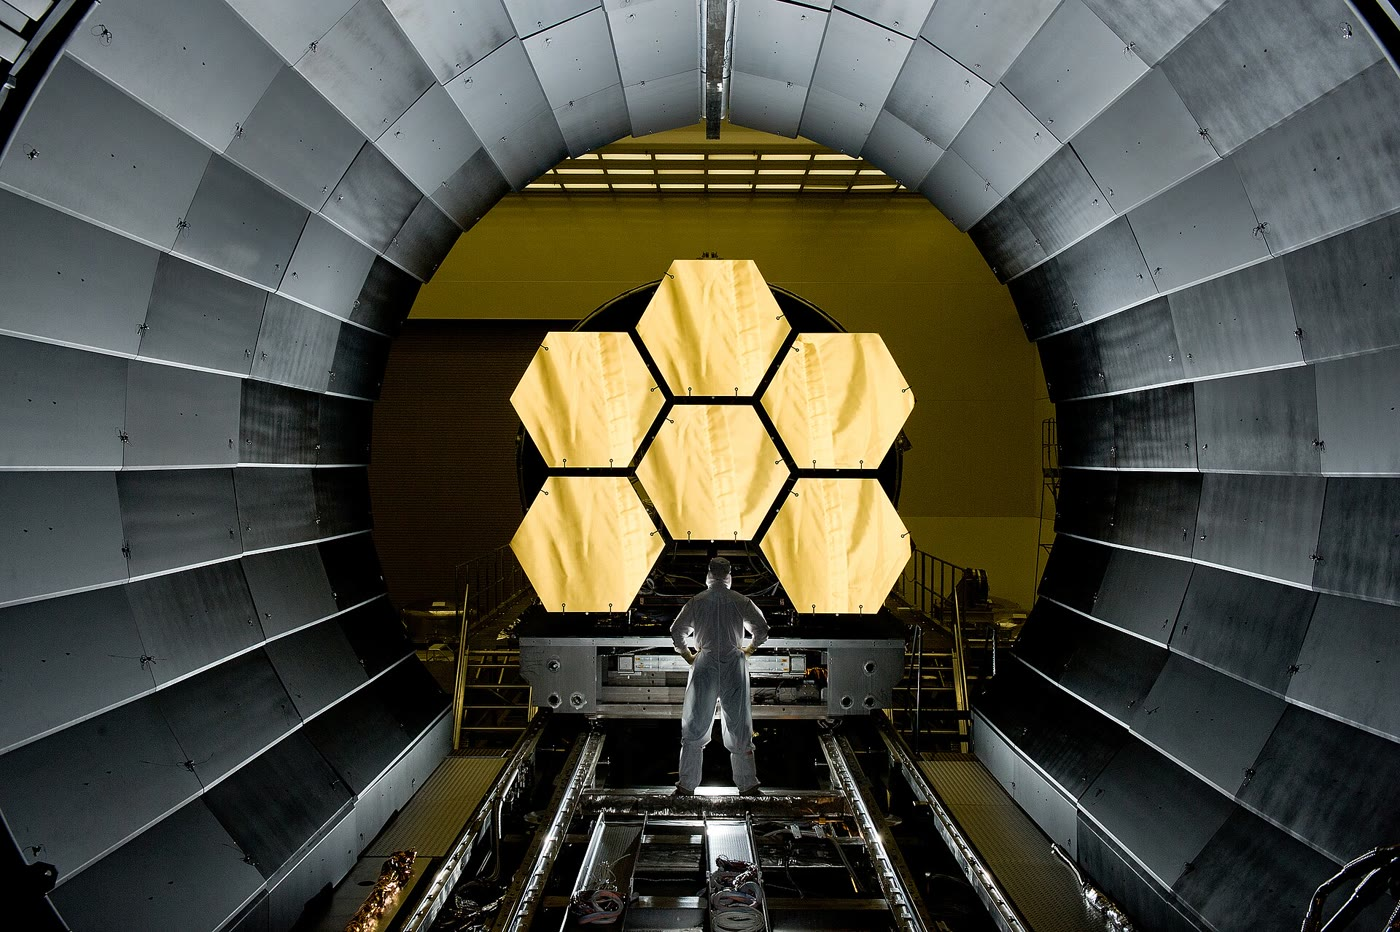
\includegraphics[width=0.78\linewidth]{images/book3/b1-jwst-mirror-segments.jpg}

{\small Enam dari 18 segmen heksagonal cermin primer Teleskop Antariksa James Webb, disiapkan untuk uji dingin pada 2011; bersama-sama, ketika dibentangkan di angkasa, ke-18 segmen itu membentuk cermin selebar \qty{6.5}{m}. Foto NASA/MSFC/David Higginbotham, domain publik.}
% ledger: commons:jwst-mirror, nasa:jwst-mirror
\end{omfigure}

\section{Latihan}

\begin{exercise}[$\star$]\label{exo:b1:observing-the-sky:1}
Berapakah perbandingan \omterm{def:b1:observing-the-sky:flux}{fluks} dua bintang bermagnitudo 1.0 dan 6.0? Berapakah perbandingan \omterm{def:b1:observing-the-sky:flux}{fluks} Rigel ($V = 0.13$) dan Polaris ($V = 2.02$)? Mana yang lebih terang di langit?
\end{exercise}

\begin{exercise}[$\star$]\label{exo:b1:observing-the-sky:2}
Paralaks Altair adalah \ang{;;0.19495}. Berikan jaraknya dalam \omterm{def:b1:observing-the-sky:parallax}{parsek}, dalam satuan astronomi, dan dalam tahun cahaya.
\end{exercise}

\begin{exercise}[$\star$]\label{exo:b1:observing-the-sky:3}
Hitunglah batas difraksi teleskop antariksa \qty{2.4}{m} pada \qty{550}{nm}, dalam detik busur, dan bandingkan dengan \omterm{def:b1:observing-the-sky:seeing}{kekaburan} \ang{;;0.40}. Lakukan hal yang sama untuk teleskop \qty{6.5}{m} pada \qty{2.0}{\micro\metre}.
\end{exercise}

\begin{exercise}[$\star$]\label{exo:b1:observing-the-sky:4}
Dari tabel empat bintang terang, urutkan Rigel, Altair, Polaris dan Betelgeuse dari permukaan yang paling panas sampai yang paling dingin. Mengapa \omterm{def:b1:observing-the-sky:colour-index}{indeks warna} dapat dibandingkan antarbintang yang berjarak sangat berbeda?
\end{exercise}

\begin{exercise}[$\star\star$]\label{exo:b1:observing-the-sky:5}
Sebuah bintang diukur bermagnitudo 6.412 pada jarak \omterm{def:b1:spherical-astronomy:celestial-sphere}{zenit} \ang{30} dan 6.590 pada \ang{60} pada malam yang sama. Dengan mengasumsikan atmosfer sejajar-bidang, hitunglah kedua \omterm{def:b1:observing-the-sky:extinction}{massa udara}, koefisien ekstingsi, dan magnitudo bintang di atas atmosfer.
\end{exercise}

\begin{exercise}[$\star\star$]\label{exo:b1:observing-the-sky:6}
Sebuah bintang memberikan 400 fotoelektron dalam pemaparan \qty{10}{s}, dan derau foton dari bintang itu sendiri mendominasi. Berapakah \omterm{def:b1:observing-the-sky:detector}{rasio sinyal terhadap deraunya}? Berapa lama harus memaparkan untuk mencapai SNR 100? Berapa lama untuk mengukur magnitudonya hingga galat \num{0.01}?
\end{exercise}

\begin{exercise}[$\star\star$]\label{exo:b1:observing-the-sky:7}
Rigel memiliki $V = 0.13$ dan paralaks \ang{;;0.00378}. Dengan mengabaikan ekstingsi antara bintang itu dan kita, hitunglah jaraknya, \omterm{def:b1:observing-the-sky:absolute}{magnitudo mutlaknya}, dan \omterm{def:b1:observing-the-sky:flux}{luminositasnya} dalam V dalam satuan Matahari ($M_\odot = 4.83$).
\end{exercise}

\begin{exercise}[$\star\star$]\label{exo:b1:observing-the-sky:8}
Bandingkan luas pengumpulan cermin lingkaran \qty{2.4}{m} (abaikan sumbatan pusatnya) dengan luas teleskop Webb (\qty{25}{m^2}). Berapa kali lebih pendek pemaparan yang diperlukan teleskop Webb untuk mengumpulkan jumlah foton yang sama? Berapa pecahan dari cakram penuh berdiameter \qty{6.5}{m} yang diwakili luas pengumpulannya, dan mengapa nilainya kurang dari satu?
\end{exercise}

\begin{exercise}[$\star\star$]\label{exo:b1:observing-the-sky:9}
(a) Dari \omterm{def:b1:observing-the-sky:flux}{luminositas} Matahari, \qty{3.828e26}{W}, hitunglah \omterm{def:b1:observing-the-sky:flux}{fluksnya} pada \qty{10}{\parsec}. (b) \omterm{def:b1:observing-the-sky:magnitude}{Magnitudo tampak} dan mutlak Matahari adalah $-26.74$ dan $4.83$. Gunakan \omterm{def:b1:observing-the-sky:absolute}{modulus jarak} untuk memperoleh kembali jarak Matahari--Bumi, dalam satuan astronomi.
\end{exercise}

\begin{exercise}[$\star\star\star$]\label{exo:b1:observing-the-sky:10}
Tunjukkan dari \cref{prop:b1:observing-the-sky:bouguer} bahwa $k =
2.5\log_{10}e\;\tau_0$. Untuk malam garis ekstingsi ($k =
\num{0.160}$), hitunglah kedalaman optik \omterm{def:b1:spherical-astronomy:celestial-sphere}{zenit} $\tau_0$ dan pecahan cahaya yang mencapai teleskop di \omterm{def:b1:spherical-astronomy:celestial-sphere}{zenit} dan pada $X = 2.31$. Apa yang akan diprediksi atmosfer sejajar-bidang untuk \omterm{def:b1:observing-the-sky:extinction}{massa udara} pada jarak \omterm{def:b1:spherical-astronomy:celestial-sphere}{zenit} \ang{85}, dan mengapa nilai itu tidak boleh dipercaya?
\end{exercise}

\begin{exercise}[$\star\star\star$]\label{exo:b1:observing-the-sky:11}
Sebuah galaksi redup memberikan $R = 50$ fotoelektron per detik di teleskop, dan langit di dalam luas citranya memberikan $B = \num{2000}$ per detik ketika \omterm{def:b1:observing-the-sky:seeing}{kekaburannya} \ang{;;0.80}. Derau baca dapat diabaikan. (a) Berapa lama harus memaparkan untuk SNR 10? (b) Langit dalam citra bertambah sebanding dengan luas cakram \omterm{def:b1:observing-the-sky:seeing}{kekaburan}. Ulangi untuk \omterm{def:b1:observing-the-sky:seeing}{kekaburan} \ang{;;0.40}. (c) Tunjukkan bahwa, untuk sumber yang jauh lebih redup daripada langit, waktu pemaparan yang diperlukan untuk SNR tertentu berubah sebagai $\theta^2/D^2$, dengan $\theta$ \omterm{def:b1:observing-the-sky:seeing}{kekaburan} dan $D$ diameter teleskop.
\end{exercise}

\begin{exercise}[$\star\star\star$]\label{exo:b1:observing-the-sky:12}
Sebuah kisi dengan 1200 garis per milimeter disinari sepanjang \qty{100}{mm} dan dipakai pada orde pertama. (a) Berapa daya resolusinya, dan berapa selisih panjang gelombang terkecil yang dapat dipisahkan pada \qty{550}{nm}? (b) Kecepatan radial apa yang sesuai dengan selisih itu? (c) Bumi mengelilingi Matahari dengan kecepatan \qty{29.78}{km.s^{-1}}. Berapa besar gerak itu dapat menggeser garis pada \qty{550}{nm}, dan berapa elemen resolusi itu? Apa yang karena itu harus dilakukan pengamat yang mengukur kecepatan bintang?
% ledger: earth:vorb
\end{exercise}

\section{Soal: Menimbang cahaya Sirius}

\begin{problem}[{Soal akhir pekan --- seberapa jauh Sirius, seberapa terang ia tampak dan berapa banyak foton yang dikirimkannya, serta berapa banyak matahari yang dikalahkannya dalam kecerlangan}]
\label{pb:b1:observing-the-sky:1}
% ledger: simbad:sirius, simbad:vega, simbad:sirius-b, nasa:sun-V, sun:Mabs, const:au
% numbers computed in the scratch calculator calc/ch02.py from the rounded data
Sirius, bintang paling terang di langit malam, memiliki pendamping redup, katai putih Sirius~B. Gunakan data berikut:
\begin{center}
\small
\begin{tabular}{lcc}
\hline
objek & $V$ & paralaks \\
\hline
Sirius & $-1.46$ & \ang{;;0.37921} \\
Sirius B & $8.44$ & --- \\
Vega & $0.03$ & \ang{;;0.13023} \\
Matahari & $-26.74$ & --- \\
\hline
\end{tabular}
\end{center}
dengan $M_\odot = 4.83$ dalam V, $\qty{1}{\parsec} = \qty{206265}{\au} =
\qty{3.0857e16}{m} = \qty{3.2616}{\lightyear}$, dan koefisien ekstingsi $k = 0.15$ per \omterm{def:b1:observing-the-sky:extinction}{massa udara} di observatorium.

\medskip
\noindent\textbf{Bagian I --- Seberapa jauh Sirius?}
\begin{enumerate}
  \item Hitunglah jarak Sirius dalam \omterm{def:b1:observing-the-sky:parallax}{parsek}.
  \item Nyatakan dalam satuan astronomi dan dalam meter.
  \item Nyatakan dalam tahun cahaya. Berapa lama lalu cahaya yang kita lihat malam ini meninggalkan Sirius?
  \item Dalam setahun, dengan sudut total berapakah arah Sirius berayun dari sisi ke sisi? Bandingkan dengan \omterm{def:b1:observing-the-sky:seeing}{kekaburan} \ang{;;0.40}. Mengapa ayunan itu masih dapat diukur hingga pecahan kecil dari \omterm{def:b1:observing-the-sky:seeing}{kekaburan}?
  \item Jika paralaksnya keliru sebesar \ang{;;0.001}, dengan pecahan berapakah jaraknya keliru, dan berapa tahun cahaya?
\end{enumerate}

\medskip
\noindent\textbf{Bagian II --- Seberapa terang ia tampak?}
\begin{enumerate}[resume]
  \item Hitunglah perbandingan \omterm{def:b1:observing-the-sky:flux}{fluks} Sirius dan Vega dalam V.
  \item Hitunglah perbandingan \omterm{def:b1:observing-the-sky:flux}{fluks} Matahari dan Sirius.
  \item Hitunglah perbandingan \omterm{def:b1:observing-the-sky:flux}{fluks} Sirius dan Sirius~B.
  \item Dari Observatorium Paranal, Sirius melintasi meridian pada tinggi \ang{82.09} (\cref{ch:b1:spherical-astronomy}). Hitunglah \omterm{def:b1:observing-the-sky:extinction}{massa udaranya}, ekstingsinya, dan magnitudo yang diukur pada saat itu.
  \item Ulangi pada tinggi \ang{30}. Berapa pecahan cahaya yang hilang di perjalanan?
  \item Mengapa rumus $X = \sec z$ dapat menyesatkan pengamat yang mengukur Sirius tepat setelah terbit?
\end{enumerate}

\noindent\textbf{Bagian III --- Menghitung foton.}
Sebuah kamera pada teleskop \qty{1}{m} merekam $\num{3.0e4}$ fotoelektron per detik dari sebuah bintang bermagnitudo $V = 10.0$, setelah dikoreksi ekstingsi. Setiap piksel menampung paling banyak $\num{1.0e5}$ elektron (kapasitas penuhnya).
\begin{enumerate}[resume]
  \item Berapa fotoelektron per detik yang direkam kamera dari Sirius~B?
  \item Berapa lama pemaparan yang memberi Sirius~B SNR 1000, dengan derau foton dari bintang itu sendiri? Berapa galat magnitudonya kemudian?
  \item Berapa fotoelektron per detik yang direkam kamera dari Sirius?
  \item Jika \qty{20}{\percent} cahaya Sirius jatuh pada piksel terterangnya, berapa lama piksel itu terisi penuh?
  \item Pada citra, sayap redup citra Sirius menyimpan, di tempat Sirius~B, $10^{-4}$ cahaya Sirius per piksel, dan piksel terterang Sirius~B mengumpulkan \qty{20}{\percent} cahayanya sendiri. Bandingkan kedua laju di piksel itu.
  \item Berapa pemaparan terpanjang yang tidak membuat piksel itu jenuh? Hitunglah SNR Sirius~B di piksel itu dalam pemaparan \qty{0.5}{s}, dengan memperhitungkan derau foton kedua sumber. Apakah Sirius~B dapat dideteksi, dan apa yang membuatnya sulit?
\end{enumerate}

\noindent\textbf{Bagian IV --- Berapa banyak matahari?}
\begin{enumerate}[resume]
  \item Hitunglah \omterm{def:b1:observing-the-sky:absolute}{modulus jarak} Sirius.
  \item Turunkan \omterm{def:b1:observing-the-sky:absolute}{magnitudo mutlak} Sirius dalam V, hingga dua desimal.
  \item Hitunglah jarak dan \omterm{def:b1:observing-the-sky:absolute}{magnitudo mutlak} Vega.
  \item Manakah di antara Sirius dan Vega yang secara intrinsik lebih terang dalam V, dan dengan faktor berapa?
  \item Berapakah \omterm{def:b1:observing-the-sky:magnitude}{magnitudo tampak} Matahari jika dilihat dari jarak Sirius? Dengan menganggap 6.0 sebagai magnitudo terredup yang terlihat dengan mata telanjang pada malam yang gelap, apakah ia akan terlihat?
  \item Sampai jarak berapakah Sirius akan tetap terlihat dengan mata telanjang?
  \item Hitunglah \omterm{def:b1:observing-the-sky:flux}{luminositas} Sirius dalam V dalam satuan Matahari: berapa banyak matahari yang dikalahkan Sirius dalam kecerlangan?
\end{enumerate}
\end{problem}
